\documentclass[a4paper,twoside]{article}

\usepackage{epsfig}
\usepackage{subcaption}
\usepackage{calc}
\usepackage{amssymb}
\usepackage{amstext}
\usepackage{amsmath}
\usepackage{amsthm}
\usepackage{multicol}
\usepackage{xcolor}
\usepackage{pslatex}
\usepackage{hyperref}
\usepackage{apalike}
\usepackage{url}
\usepackage{booktabs}
\usepackage{SCITEPRESS}     % Please add other packages that you may need BEFORE the SCITEPRESS.sty package.


\begin{document}

\title{Assessing the importance of global relationships for source code modeling using Graph Neural Networks}

% \author{\authorname{Vladimir Ivanov\orcidAuthor{0000-000x-xxxx-xxxx}, Vitaly Romanov\orcidAuthor{0000-000x-xxxx-xxxx}, Giancarlo Succi\orcidAuthor{0000-0001-8847-0186}
% }
% \affiliation{\sup{1}Innopolis University, Russia}
% \email{\{f.last\}@innopolis.ru}
% }

\keywords{source code, graph, neural networks, graph attention networks, relational graph convolutional networks, graph neural networks}

\abstract{
Modern approaches for source code analysis usually represent the source code as a sequence tokens. Such representation cannot capture long-distance dependencies in the source code and inter-project dependencies. The usefulness of such relationships between entities in the source code for solving machine learning tasks is an open question addressed in this paper. In this study, we analyze to which extent inter-project relationships can be used in machine learning tasks related to source code analysis. Our findings show that information implicitly stored in inter-project relationships can be used to select the next called function among candidates with an accuracy of 92\%. We demonstrate that source code embeddings computed with GNNs achieve the best performance on transfer learning tasks when trained on multiple objectives simultaneously. 
% We represent source code in the form of a graph. In this graph, nodes are entities in source code, such as modules, classes, methods, and functions. The edges are inter-project relationships that represent imports, function calls, definitions, etc. 
% The information about the definitions of functions and methods seem to affect the performance of our models the most. 
% We find that embeddings for nodes in the global graph trained with GNNs can be used for solving other tasks as well. 
%  suggest that information about inter-project relationships is valuable for augmenting other source code representations.
}

\onecolumn \maketitle \normalsize \setcounter{footnote}{0} \vfill

\section{\uppercase{Introduction}}
% \noindent 
Source code can be viewed as a form of natural language. Lately we see the rise of the approaches that try using advances in the area of Natural Language Processing to solve machine learning tasks for source code. One of the noteworthy applications of modeling source code is the source code search. In this application, a user can find a relevant code snippet using a natural language query. Such approaches do not even require the code to have any extra annotation or documentation. However, most of such approaches work on the level of the body of a single function, which, in most cases, is sufficient to understand the purpose of this function. However, learning algorithms still struggle to process sequences of actions that are common in source code. At the same time, current approaches proved to be quite successful in capturing co-occurrence statistics. For source code, such statistics can be extracted from global usage patterns on a package or inter-project levels. Our goal is to study how useful this global information is by posing this goal as an evaluation of machine learning tasks on graphs.
 
Source code describes the relationships between source code objects (SCOs), such as modules, functions, classes, variables, etc. Some information about these SCOs can be inferred from the package and inter-project level dependencies. A package contains information about the contextual similarity. The SCOs from the same package are likely to have a related purpose. The information about how particular SCOs are used in different projects can tell us which packages are often used together, and what are the common combinations of SCOs to be used together in various projects. On these levels of abstraction, one does not concern with the particular way an SCO is implemented and can learn useful insights about its purpose from merely observing the way it is used. Traditional NLP approaches are not suited to capture these kinds of relationships because they treat the input as a sequence of tokens. A structured representation of the source code is required instead.

The package and inter-project levels of abstraction are well represented using a graph. Such a graph can include different types of relationships, including call dependencies, type dependencies, import dependencies, variable usages, inheritance dependencies, and others. Because the relationships between SCOs are not constrained to the boundaries of particular functions, files, and even packages, such a graph captures global relationships, and, therefore, is a global graph. Global graph representation is an alternative approach to represent the source code besides other structures representations, such as abstract syntax trees (ASTs). We evaluate the usefulness of this global graph representation by solving different machine learning problems for source code. In this work, we aim at assessing what kind of information can be inferred from high-level inter-project global relationships between SCOs. Moreover, we look into the transferability of learned distributed representations for nodes in this graph to other problems. We purposefully do not consider the ASTs as their study was addressed in other works \cite{Alon2018}, \cite{Yahav2018}.

Several papers investigated what a model can learn from a particular source code representation. \cite{Alon2018a} used AST paths to predict the names of functions. \cite{Allamanis2017} used graph representation that relies on both global relationships and ASTs to find bugs. \cite{DeFreez2018} used an inter-procedural flow graph to find similar functions inside the Linux kernel source code. \cite{Raychev2015} used information about AST to predict variable names and types within a function. In contrast to these works, we focus on using only information about global relationships. 

Our contribution is the following
\begin{itemize}
    \item We introduce a source-graph-dataset that captures information about global relationships between over 100 Python packages\footnote{link will be added in camera-ready version};
    \item We evaluate the usefulness of a global graph on several machine learning tasks, including SCO name prediction, variable name usage prediction, API call sequence prediction. For our experiments we use Graph Neural Networks (GNNs);
    \item We explore the usefulness of multitask objective using different GNN architectures
    \item We demonstrate that the embeddings for SCOs pre-trained on one task can be applied to solve other tasks such as function call prediction, type use prediction, node type prediction;
    \item We assess the importance of different types of edges in the global graph for successfully learning an objective. 
\end{itemize}

The rest of the paper is organized as follows. In Section~\ref{sec:related} we overview related work. In Section~\ref{sec:main} we discuss the main training objectives and our GNN models. In Section~\ref{sec:training} we explain our GNN training process. In Section~\ref{sec:experiments} we explain our experiments for assessing transfer learning. In Section~\ref{sec:setup} we state our choice of hyper-parameters and explain our experimental observations. In Section~\ref{sec:discuss} we explain some of our design choices. Section~\ref{sec:conclusion} concludes the paper.

\section{\uppercase{Related Work}}\label{sec:related}

Machine learning approaches are rapidly adopted in many different areas, including solving problems in source code analysis. The list of problems that were already attempted include tasks such as bug detection \cite{Dinella2020} \cite{Wang2019} and API search \cite{Zhang2019} \cite{Wan2019}. These problems present a fundamental challenge for methods of source code analysis because they require the understanding of the program purpose. Other applications include type prediction \cite{Hellendoorn2018} \cite{Malik2019}, variable name prediction \cite{Cvitkovic2018} \cite{Bichsel2016}, function name prediction \cite{Lacomis2019} \cite{Alon2018}, program classification \cite{Ben-Nun2018} \cite{Zhou2019} \cite{Dam2019}, program summarization \cite{Fernandes2019} \cite{Shido2019} and other \cite{Nguyen2015} \cite{Yang2019} \cite{Chen2019} \cite{Drissi2018}.  

One important aspect of learning problems is the representation of the input data. In the area of NLP the input is represented as a sequence. Although the source code is a sequential representation of a program, its execution nature is far from sequential. For this reason, researchers explored more suitable representation formats for source code. Here, we consider structural representation such as trees (ASTs) and graphs (dependence, control-flow, data-flow, etc). One of the valid research questions is which representation formats are useful for solving different target problems. Despite some progress, the research into representation formats for machine learning on source code is still ongoing.

\cite{Raychev2015} represent a program in the form of AST\@. They try to address the problem of predicting variable names in an obfuscated program. Such a program can be either obtained in the process of decompilation or from obscured sources. Their approach, based on CRF, was highly successful, and their method was able to annotate the names of the variables by only analyzing the program structure. The input of the analyzer is a whole function. This approach provides an insight into the information that is implicitly stored inside a program's AST\@.

AST might be useful for predicting variable names, but it is not guaranteed to be useful for other problems. In~\cite{Alon2018}, an approach for using AST paths for predicting function names was introduced. Their approach was successful in predicting function names for Java code snippets. According to the authors' claim, the result appeared to be better than in~\cite{Raychev2015}. In this work, a comprehensive comparison of different approaches to predict variable names was performed. The authors showed that AST path-based representations are useful to characterize a large portion of code, such as an entire function. 

Some researchers turned towards Graph Neural Networks (GNNs). In~\cite{Allamanis2017}, graph-based representation of C\# source code was studied. The authors used both global-level relationships as well as AST edges. This graph included such relationship edges as inheritance, definitions, variable uses, and typical data flow information that can be extracted from an AST\@. Authors used GNNs to address issues in source code analysis, such as variable name suggestion and bug detection. 
Another approach that adopted graph representation for source code was presented in~\cite{Cvitkovic2018}. They used information from AST and global relationships for the variable name suggestion problem. These two works combine AST of functions with inter-project information, but they do not study the role of different relationships in the final result. 

Some other approaches they rely on the information from the LLVM compiler to build graph representations \cite{Ben-Nun2018} \cite{Brauckmann2020}. However, such representations are available only for a handful of programming languages and, in general, are less interpretable. In contrast, our goal is to perform the analysis on the level of source code directly, so that a programmer can easily interpret the results. 
% For this reason we will not go into depth describing these other approaches.

The research in source code representation formats for machine learning is ongoing. In this regard, our contribution is in exploring to which extent the global relationships in the source code are useful for predicting some of the properties of SCOs.

Another important aspect of machine learning models is the transferability of knowledge. Transfer learning is widely used in the area of NLP, where representations for words are pre-trained using either unsupervised objectives (such as ones used for Skipgram or BERT).
% Different forms of pre-training for the source code were studied as well. 
In \cite{Kanade2019}, authors studied the possibility of pre-training representations for the source code using one of the latest language modeling tools --- BERT\@. Their result have shown that when using pre-trained layers, the model quickly adapts to the new problem and provides a significant boost in performance. Authors demonstrated, that pre-training with a language model can significantly decrease training times and increase accuracy. We are interested in a different aspect of pre-training. Given an objective function, the model learns useful features for this objective. However, the same features can be helpful for other objectives as well. Our goal is to investigate to which extent representations of SCOs learned on one task can be used for solving other tasks.



\section{\uppercase{Main Task Description}}\label{sec:main}

\subsection{Global Graph Description}

In this work, we represent the source code with a global graph. We used the Sourcetrail\footnote{https://www.sourcetrail.com/} tool to index a collection of Python packages. All packages are interconnected either through inter-package calls and imports, or through the use of similar built-in functions from Python language. 

The entire package collection is compiled into a graph with different types of nodes and edges. The type count for nodes and edges is given in  Tables~\ref{tbl:python_node_count} and~\ref{tbl:python_edge_count} respectively.

The central aspect of our source code graph is directed typed relationships. Five different edge types are available for Python.

\begin{itemize}
    \item \textbf{Call edges}. These edges are present between two functions if one function calls another function inside its body.
    \item \textbf{Define/Contain Edges}. These edges can represent relationships between different objects. Such edges are present between modules and functions or classes that are defined in these modules. Also, these edges exist between classes and class methods.
    \item \textbf{Type use edges}. These edges appear between functions and classes to represent that a specific class (type) was mentioned inside the body of the function.
    \item \textbf{Import edges}. This relationship is registered when a module or function is imported.
    \item \textbf{Inheritance edges}. These edges are present between classes if one inherits the other. 
\end{itemize}

The nodes in our graph also have different types that are self-explanatory (see Table~\ref{tbl:python_node_count}). However, the node types were not used when training our models due to the limitation of our computational capacity. The example of a graph, compiled using Sourcetrail is shown in Figure~\ref{fig:python_graph}.

\begin{figure}
    \centering
    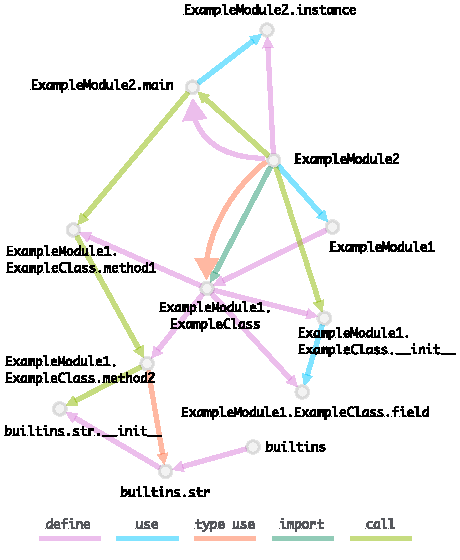
\includegraphics{python_graph_example.pdf}
    \caption{Example of global graph constructed from two toy modules.}\label{fig:python_graph}
\end{figure}

\begin{table}[]
\centering
\begin{tabular}{lll}
    \toprule
    \textbf{Node Type}        & \textbf{Count}  \\ \midrule
    Function        & 221822 \\ \midrule
    Class field     & 83077 \\ \midrule
    Class           & 35798 \\ \midrule
    Module          & 18097 \\ \midrule
    Class method    & 14953 \\ \midrule
    Non-indexed symbol  & 853  \\ \bottomrule
\end{tabular}
\caption{Node types present in Python source graph\label{tbl:python_node_count}}
\end{table}

\begin{table}[]
\centering
\begin{tabular}{ll}
\toprule
\textbf{Edge Type}       & \textbf{Count} \\ \midrule
Call            & 614621 \\ \midrule
Define/Contain  & 431115 \\ \midrule
Type use        & 239543 \\ \midrule
Import          & 121752 \\ \midrule
Inherit         & 26525 \\ \bottomrule
\end{tabular}
\caption{Edge count in Python graph by edge type\label{tbl:python_edge_count}}
\end{table}

\subsection{Description of Learning Objectives}\label{sec:objectives}

% In this paper, we pursue several goals. First, we are studying global graph representation for the source code. We do this by evaluating a GNN model trained on this graph on several tasks. 
One of our goals is to evaluate a GNN model trained on a global source graph. We do this by training this model using several objectives.

The first objective is SCO \textbf{name prediction}, which includes predicting function names, class names, variable names, etc. This objective can be seen as semantically challenging because the original graph contains only the information about the relationships between SCOs. The premise for this task is that objects with specific common names have fixed usage patterns. The fact that some objects can be references in common settings implies that they have a similar purpose, and often, similar names. In this task, the target can be defined for every node in the global graph.

The second objective is \textbf{predicting names of variables} that are used inside a function. This is also a semantically challenging task. Very often, variable names explain the purpose of a function, or at very least, the topical area to which this function belongs. We expect that functions that implement similar functionality, or belong to the same package are likely to use similar variable names. The variable names are extracted from function bodies. Because of the way the objective is specified, the target is defined only for the nodes in the graph that represent functions.  

The third objective is \textbf{predicting next function} to be called after the current function. In order to be able to predict the next call, the model should learn common usage patterns for functions. These usage patterns include built-in functions, functions from the same package, and functions from other packages. As with the case of variable name prediction, the objective is defined only for the nodes that represent functions. 

Some of the objectives are defined only for a subset of nodes. However, the GNNs are implemented in a way, where representation for all nodes are trained simultaneously. For this reason, GNN learning tasks are sometimes seen as semi-supervised learning problems.

All of three objectives can be treated as link prediction problems. During the training, embeddings for two nodes are passed to the classifier for link prediction. The two nodes specify the source and destination of a directed edge. Depending on the objective, the two nodes are taken from different groups. The source node always represent an SCO object in the global graph, and its embedding is computed using GNN\@. The second node can be either a node for SCO name, a node for the variable name, or another SCO\@. In the case of names, the embedding for the second node is drawn form a dedicated embedding table. Otherwise, it is also generated by GNN\@. The link prediction is implemented by concatenating the embeddings for the source and destination of the edge, and passing the resulting vector to a binary classifier. We implement this classifier using a simple neural network.

We use three objectives explained above to train several GNN models to see to which extent the information about global relationships is useful for solving these tasks. Moreover, we experiment with a multitask objective. After, we investigate the applicability of learned distributed representations to predict properties of some of the nodes in the global graph with a series of experiments. These experiments are designed to identify the usefulness of objectives described above for solving other tasks. The details of these experiments are given in Figure~\ref{fig:model}.

\begin{figure*}
    \centering
    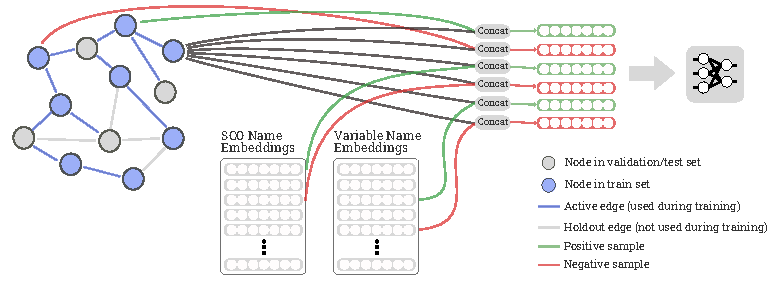
\includegraphics[width=\textwidth]{model.pdf}
    \caption{Schematic representation of the multitask training procedure training procedure. The final neural networks makes a binary decision whether the edge exists or not.}
    \label{fig:model}
\end{figure*}

\subsection{GNN Models}

Graph Neural Networks (GNN) is based on a message-passing mechanism. Each node possesses an internal state. During message-passing, the node sends its state to its neighbors. The neighbors aggregate messages from adjacent nodes using a neural network. Usually, the messages are passed over the entire network for a fixed number of steps. The message-passing steps are treated as network layers. The final node state is passed to the classifier that predicts links. The initial representation of a node is a context-free embedding. Embeddings from the consecutive layers can be viewed as the contextual. The size of the context depends on the number of layers. The best context size for solving the link prediction task is subject to exploration.

In our experiments, we use two different GNN architectures. The first is the Graph Attention Network (GAT). This architecture does not support different types of relationships and treats them the same. The second architecture is Relations Graph Convolutional Network (RGCN). This network was designed to process heterogeneous graphs and supports different types of edges. We use these two types of networks to investigate the impact of the edge types on the final result. 

Other works that rely on GNNs use more complicated architectures \cite{Allamanis2017} \cite{Cvitkovic2018}. However, the search of the best neural architecture is not our goal. For the latest findings in the area of architecture search for processing source code with GNNs see \cite{hellendoorn2020global}.

The reason we choose GNN models for our experiments is because, at the moment, they are considered the most suitable for processing graphs. 
We tried to use other approaches for learning representations for nodes, specifically Node2Vec, but they did not prove to be useful for out tasks.

% \textbf{Graph Attention Network} is a model that uses the attention mechanism during the aggregation of messages. Thus, this neural network can select the most relevant messages for computing the current internal state.

% $$
% h_i^{(l+1)}=\sigma\left(\sum_{j\in \mathcal{N}(i)} {\frac{1}{c_{ij}} W^{(l)}h^{(l)}_j}\right)
% $$

% \textbf{Relational Graph Convolutional Network} allows modeling heterogeneous graphs with different relation types. In this variant, there is a dedicated set of weights for each type of connection. 
% $$
% h_i^{(l+1)} = \sigma\left(\sum_{r\in \mathcal{R}}
% \sum_{j\in\mathcal{N}_r(i)}W_r^{(l)}h_j^{(l)}\right)
% $$


\section{\uppercase{GNN Training Procedure}}\label{sec:training}

In the process of training a GNN model on one of the objectives, embeddings for graph nodes are learned. These embeddings are used in several scenarios. First, they are passed to the classifier that predicts links for the main objective. Second, they are used in further experiments with transfer learning. Because of this setting, the optimization of the main objective can be seen as the pre-training step. The assessment of transfer learning requires training additional models on parts of the same graph.

Due to the need to evaluate the usefulness of the learned embeddings for the transfer learning, a careful pre-processing procedure for splitting data into train and test sets should be used. This procedure helps to ensure that the training signals do not leak into the test data. In this section, we are going to explain:
\begin{itemize}
    \item The pre-processing procedure for the global graph
    \item What is the train-test splitting policy for training the main objective
    \item How does pre-training procedure looks
    \item What is the list of experiments for assessing the transferability of learned embeddings
\end{itemize}

The entire training and testing procedure is shown schematically in Figure~\ref{fig:splits}.

\begin{figure}[]
    \centering
    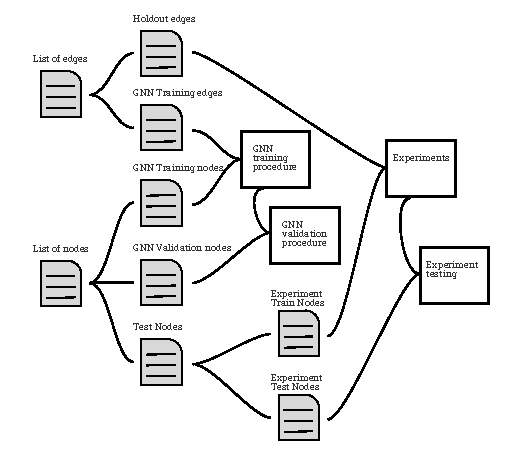
\includegraphics[width=\columnwidth]{splits.pdf}
    \caption{Schematic representation of training procedure. Should be read from left to right. First, GNN model is trained. Then, experiments are conducted on the test set and holdout edges.}\label{fig:splits}
\end{figure}

\subsection{Dataset Splits for Training and Evaluation}\label{sec:splits}

The global graph is prepared in the following way:
\begin{enumerate}
    \item Edges are split into the train set and holdout set. The holdout set is used in future experiments. Without a holdout set, the results of future experiments may be biased. After removing holdout edges from the main graph, the disconnected nodes are filtered, so that the graph remains connected. The fraction of the holdout edges is 10\% of the total.
    \item Training objectives will be defined based on node embeddings. For this reason, the train, test, and validation sets are creating splitting on nodes. The test set is used in future experiments for training and testing. Validation and test sets are equal in size and constitute 40\% of all nodes.
\end{enumerate}

\subsection{GNN Training Procedure}\label{sec:gnn_training}

As it was mentioned above, the nodes are split into three groups: train, validation and test sets. As it was described in Section~\ref{sec:splits}, the goal is to predict the presence of a link between the source and destination nodes. During the training, only positive samples are available in the dataset. The negative samples are generated randomly. When preparing a batch for training, we take source nodes from the train set. Then, we sample the positive edges that are available for these nodes in the global graph. After, we generate negative edges by sampling destination nodes using the negative sampling procedure from~\cite{mikolov2013distributed}. The fact that the graph edges are split into the train and validation sets based on the source node allows the link prediction classifier to observe all the connections of a specific node. Then, it can transfer its knowledge onto the edges with source nodes that it has never observed before.

The evaluation of the quality of the model is performed similarly. We take nodes from the validation set, and take all positive edges for these nodes. In addition, we generate negative edges using the negative sampling procedure describe above. The number of positive and negative samples is equal. We assess the quality of the model using accuracy. This way, the accuracy of the random baseline is 0.5.

\section{\uppercase{Experiments for Transfer Learning}}\label{sec:experiments}

One of our goals is to study the transferability of learned representations for nodes onto different tasks. For this reason, we use embeddings trained using objectives described in Section~\ref{sec:objectives} for predicting some of the properties of these nodes. All of the properties are posed as link prediction problems. In fact, the experiments described below help to assess how useful learned node embeddings are for predicting other links in the global graph. The list of experiments include:
\begin{enumerate}
    \item \textbf{Predicting SCO name} 
    This task is the exact copy of one of the objectives of the main task. If the main objective was to predict SCO names, it is expected that this experiment should show nearly identical performance. Moreover, this task allows to evaluate whether embeddings trained on predicting next calls are useful for predicting names as well. 
    \item \textbf{Predicting variable name usages}
    The goal of this task is to predict variable names that were used inside a given function.
    \item \textbf{Predicting next function}.
    In this experiment, the task is to predict the edge between functions A and B, that shows that B was called after function A. 
    \item \textbf{Predicting call links}. 
    In this experiment, the goal is to predict the existence of call edges between two nodes. Training data is taken from the holdout set that contains edges that were not used during training. 
    \item \textbf{Predicting type usage}.
    The edges for type use are taken from the holdout edges. These edges show that the specific type (class) was mentioned inside the body of some function. 
    \item \textbf{Predicting node types}.
    In this procedure, a simple node embedding classifier is applied. This procedure does not require to predict the interaction between two nodes and requires only one node embedding as an input. 
\end{enumerate}

The training procedure for the experiments listed above resembles the procedure for training the main objective that was described in Section~\ref{sec:gnn_training}. The experiments are performed only on nodes that were previously reserved for the test set. The embeddings for nodes were precomputed previously using GNN and now are retrieved using an embedding table. The embeddings for the SCO nodes remain unchanged during the experiments. This ensures that we test what can be extracted from these embeddings instead of using them merely for initialization. 

We take the test set of nodes that was generated during the preparation of the main objective. We split this set into the new train and test sets. Then, the SCO embeddings are used for link prediction. It is worth noting that we train embeddings for names (including variable names) and the link prediction classifier from scratch. The summary of what is trained for each experiment is shown in Table~\ref{tbl:experiment_desc}.

\begin{table*}
    \centering
    \caption{Description of experiments and what is trained}\label{tbl:experiment_desc}
    \begin{tabular}{p{3cm}p{6cm}p{5cm}}
    \toprule
        \textbf{Experiment} & \textbf{Model description} & \textbf{What is trained} \\ \midrule
        Next function, Function call, Type usage & Both nodes have pre-trained embeddings. Node embeddings are concatenated and classified & Binary classifier for link prediction \\ \midrule
        SCO name, variable name usage & Source node embedding is pre-trained, destination node embedding is trained from scratch. & Binary classifier. Embeddings for destination nodes. \\ \midrule
        Node type & Node embedding is classified into a relatively small number of classes. Node embedding are pre-trained. & Node classifier \\ \bottomrule
    \end{tabular}
\end{table*}



\section{\uppercase{Experimental Setup and Results}}\label{sec:setup}

For implementing GNN training procedure, we use DeepGraphLibrary\footnote{https://www.dgl.ai/}. We use standard implementations of GAT and RGCN networks. For GAT, we use the size of the hidden representation of 50 with two-head-attention. This yields hidden state representation of size 100. In all layers, we use LeakyReLU as activation because, according to our observations, it produced the best results for this type of GNN\@. For RGCN, we use the size of hidden layers equal to 100. HardTanh was chosen as the activation function. Both network types have three layers in total. 

The embeddings for SCO names and variable names reside in separate embedding tables. In both cases, they have embeddings of size 100. We use a simple neural network as a binary classifier. Since it accepts concatenated vectors as input, the input dimensionality is 200. This network has one hidden layer with 20 units. ReLU was chosen as the activation function for the classifier layers. The dimensionality of embeddings and the hyper-parameters of the binary classifier are identical during additional experiments. We trained GNN models for 60 epochs.

The negative sampling procedure is similar to the one used in \cite{mikolov2013distributed}. The noise distribution is created from raised unigram distribution computed for destination nodes. The weight of unigram distribution are taken to the power of 3/4 (as in the original Word2Vec paper). During the training of a GNN model, we sample 3 negative edges per one positive edge. During additional experiments, the number of positive and negative edges during the training is the same.

\subsection{Performance on Main Objective}

Our training and evaluation procedure consists of several steps. First, we talk about the result of training on the main objectives. The four main objectives that we explored are described in Section~\ref{sec:objectives}. 

Our GNN models struggled the most to predict SCO names. This is expected because, in general, to predict SCO names correctly, the algorithm should understand high-level information about a SCO\@. In our global graph, the only information that a predictor can use is the degree of a node in a graph, and the types of relationships. Additionally, it can get insight into a small neighborhood at a distance of 2 from the current node (based on the numbed of GNN layers). The number of different relationships is small, and the degree of a node is likely a bad predictor of SCO name. Nevertheless, the accuracy was observed to be larger for models without multitask, that optimize specifically for name prediction.

Variable name usage prediction is a much more relaxed problem. Variable names are highly reused in different contexts. The fact that two functions share many variable names in common can signify that they are likely to implement similar or related functionality. For this objective, we see a consistent improvement with the increase of the model complexity. The outcome was better for models trained on multitask objectives and models that support relationship types.

The last objective was to predict which a function that will be called next. The performance for this objective was the highest, which suggests that the models were able to learn stable call sequence paths to some degree. The outcome was better for the relational model and improved significantly when trained on the multitask objective. 

These results demonstrate that the global graph contains some information that can be used for learning API call sequences, some information about SCO names, and variable usages. It is worth mentioning that all of these problems have an ample search space. The number of unique destinations for SCO name prediction is 197625, for variable usage --- 141585, and for predicting next call --- 72869. The accuracy performance for these objectives s not very high (except for the next call predictions), which suggests that global graph relationships can be used for augmenting other representations, but are likely not sufficient on their own for solving practical problems. The summary of these results are shown in Figure~\ref{fig:main_obj}.

\begin{figure}[]
    \centering
    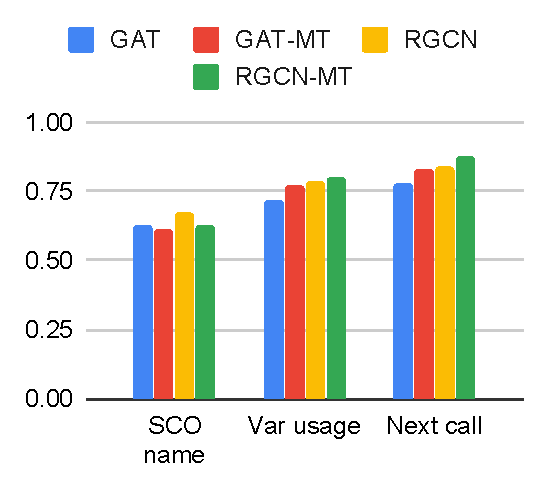
\includegraphics[width=\columnwidth]{main_objective.pdf}
    \caption{Accuracy on the validation set when training main objectives on the global graph. The color of a bar represents the model architecture that was used during training. During multitask, all three objectives are optimized at the same time.}\label{fig:main_obj}
\end{figure}

\subsection{Transfer Learning Experiments}

In this part, we are going to discuss the performance of node embeddings on transfer learning tasks. We conducted a series of experiments, and compared the performance of pre-trained embeddings with randomly initialized embeddings for SCOs. When training models for our experiments, we passed the test scores after each epoch through the exponential moving average (of length 10), and recorded only the maximum test scores. The result of these experiments for GAT are shown in Table~\ref{tbl:transfer_results}.
% Figure~\ref{fig:transfer_gat} and for RGCN --- Figure~\ref{fig:transfer_rgcn}.

For the first three experiments we can see that the accuracy is higher when the embeddings are trained on the same objective. This result is challenged only by multitask objectives. The fact that multitask objective results in the average increase of accuracy suggests that these tasks are not entirely independent.

The problem of predicting SCO names is a hard one, and the result is barely changed when a different pre-training objective is used. The results on variable usage prediction suggest that there is an improvement for both GAT and RGCN when the multitask objective is used. 

The accuracy of predicting the next call grows significantly when the multitask objective and relationship types are used. The results for predicting function calls correlate with the results of the next call prediction. 

The accuracy for predicting type usage varies a lot and does not display any specific improvements for different pre-training objectives. This can be attributed to small test size and a large variance in the test scores. Another possible explanation is a weak coupling between pre-training objectives and actual use of specific types. 

Interestingly, SCO names seem to correlate with node type (to be expected). As a consequence, all models show that node type prediction is better when pre-trained on SCO names. Another notable observation is that relationship types seem to be very important for predicting node types (also, to be expected).

Despite RGCN being conceptually superior because it supports relationship types, the results show that the difference between GAT and RGCN is very small when trained with the multitask objective. The side by side comparison of multitask models is shown in Figure~\ref{fig:mt_comparison}. 

\begin{table*}[]
\centering
\caption{Results from using pre-trained embeddings for different problems}
\label{tbl:transfer_results}
\begin{tabular}{llllllll} \toprule
\textbf{Model}  & \textbf{SCO name} & \textbf{Var usage} & \textbf{Next call} & \textbf{Call}  & \textbf{Type usage} & \textbf{Node type} & \textbf{Average} \\ \midrule
Random init     & 52.6              & 64.81              & 60.75              & 52.84          & 53.38               & 46.45              & 55.13            \\ \midrule
GAT, SCO name   & 63.6              & 74.86              & 82.29              & 65.04          & 57.81               & 65.51     & 68.18            \\ \midrule
GAT, Var usage  & 61.8              & 75.3               & 81.7               & 71.19          & 67.28               & 58.01              & 69.21            \\ \midrule
GAT, Next call  & 60.13             & 72.91              & 87.82              & 72.86          & \textbf{69.29}      & 52.6               & 69.26            \\ \midrule
RGCN. SCO name  & 63.27             & 76.28              & 86.37              & 65.07          & 64.67               & \textbf{81.84}              & 72.91            \\ \midrule
RGCN. Var usage & 63.73             & 78.33              & 89.09              & 73.24          & 68.72               & 80.9               & 75.66            \\ \midrule
RGCN. Next call & 63.02             & 76.62              & 92.22              & 74.54          & 66.76               & 77.73              & 75.14            \\ \midrule
GAT-MT          & 62.79             & 78.17              & \textbf{92.8}      & \textbf{80.03} & 65.51               & 63.43              & 73.78            \\ \midrule
RGCN-MT         & \textbf{64.48}    & \textbf{78.88}     & 91.54              & 74.44          & 63.9                & 81.62              & \textbf{75.81}  \\ \bottomrule
\end{tabular}
\end{table*}

% \begin{figure}[]
%     \centering
%     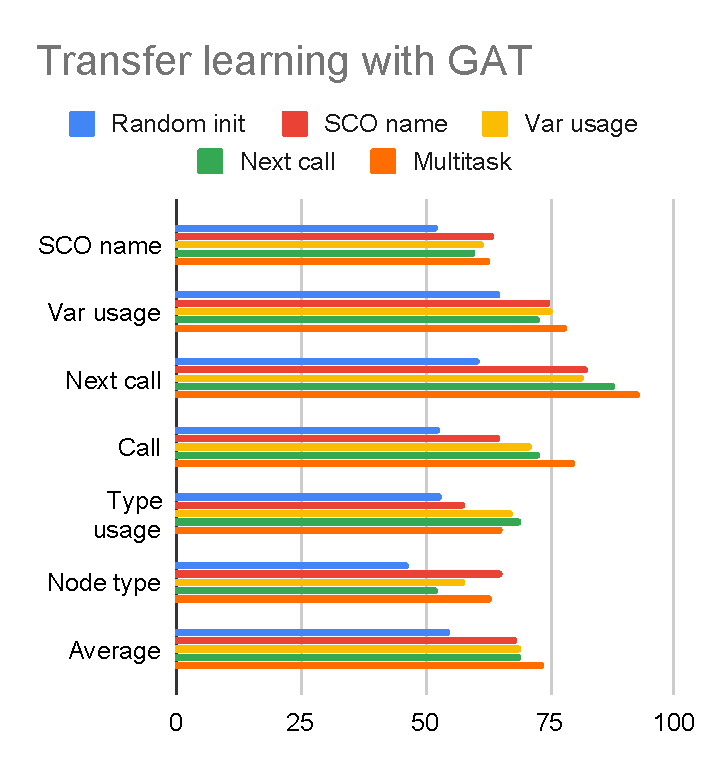
\includegraphics[width=\columnwidth]{transfer_gat.pdf}
%     \caption{Accuracy on additional experiments when using embeddings trained with GAT\@. The color of a bar corresponds to the main training objective.}\label{fig:transfer_gat}
% \end{figure}

% \begin{figure}[]
%     \centering
%     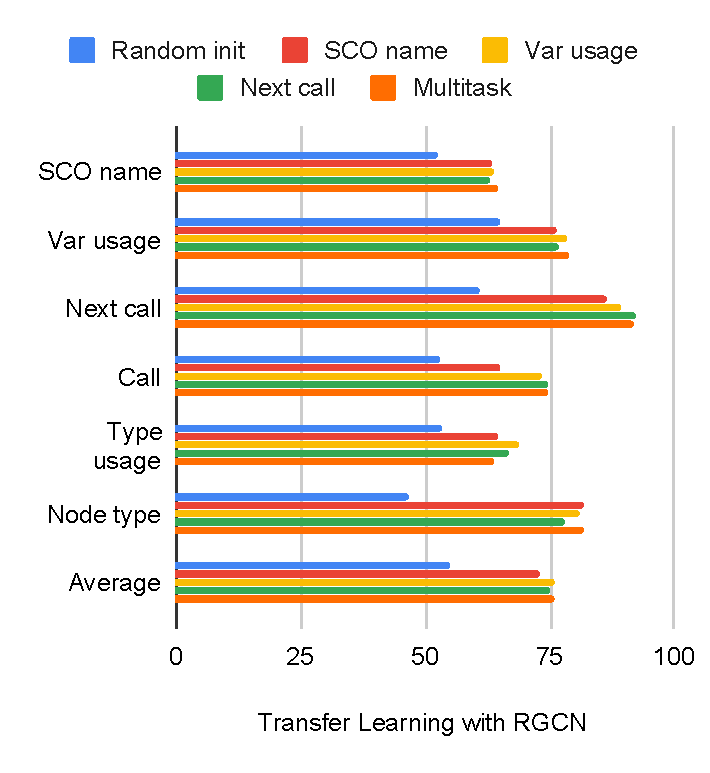
\includegraphics[width=\columnwidth]{transfer_rgsn.pdf}
%     \caption{Accuracy on additional experiments when using embeddings trained with RGCN\@. The color of a bar corresponds to the main training objective.}\label{fig:transfer_rgcn}
% \end{figure}

\begin{figure}[]
    \centering
    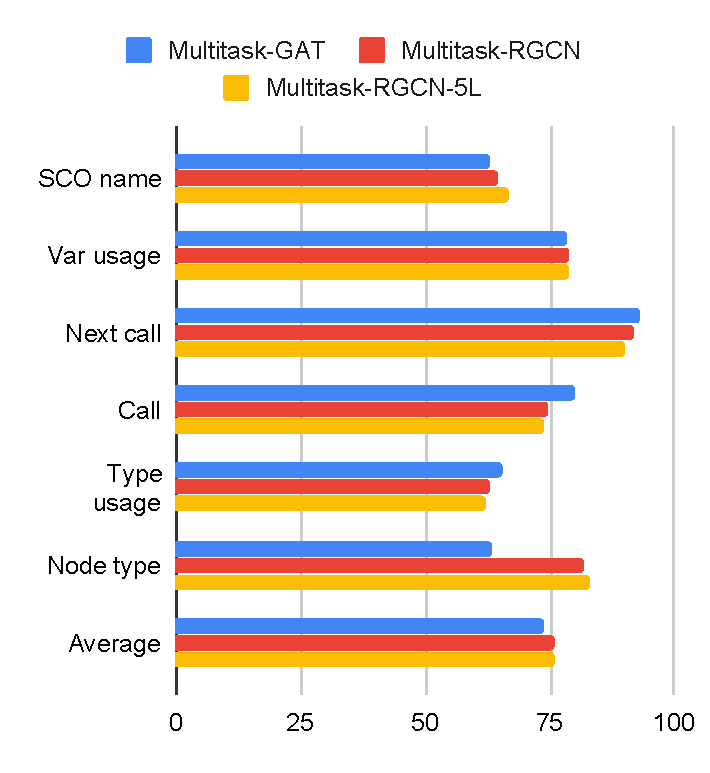
\includegraphics[width=\columnwidth]{mt_comparison.pdf}
    \caption{Accuracy comparison for different types of multitask models. RGCN-5L corresponds to a GNN model with 5 layers}\label{fig:mt_comparison}
\end{figure}

\subsection{Comparing Performance of Embeddings from Different Layers}

An intuitive question to ask is whether GNN layers provide any benefit for learning SCO embeddings. An alternative could be to optimize the embeddings for SCOs directly. We want to remind that one of the benefits of using GNNs is their robustness to partial labeling. The information from labeled nodes can propagate to unlabeled nodes. 

To investigate the value of message passing in GNN, we evaluated our experiments using embeddings from different layers of GNN\@. The results for RGCN with 3 layers are shown in Figure~\ref{fig:rgcn_layers_3}. We observe that the accuracy on different experiments improve rapidly and consistently with every layer (except type usage prediction). Three layers of GNN correspond to two message-passing steps. Therefore, a GNN with three layers can model only short distance dependencies.

Since every layer brings improvements in accuracy, a natural urge is to add more layers. However, our experiments show that adding more layers is not guaranteed to bring better results. In Figure~\ref{fig:rgcn_layers_5} the analysis of accuracy for embeddings from RGCN with five layers is shown. The average accuracy did not exceed the accuracy of the 3-layered model. Moreover, we can observe that improvements between consecutive message passing became smaller. The fact that all three models shown in Figure~\ref{fig:mt_comparison} reach similar performance (despite their architectural differences) suggests that the accuracy for these models in the current setting is close to maximum. Another explanation of why models with more layers do not achieve better accuracy is related to the general issue of GNNs to prefer a fewer number of layers \cite{zhou2018graph}.

\begin{figure}[]
    \centering
    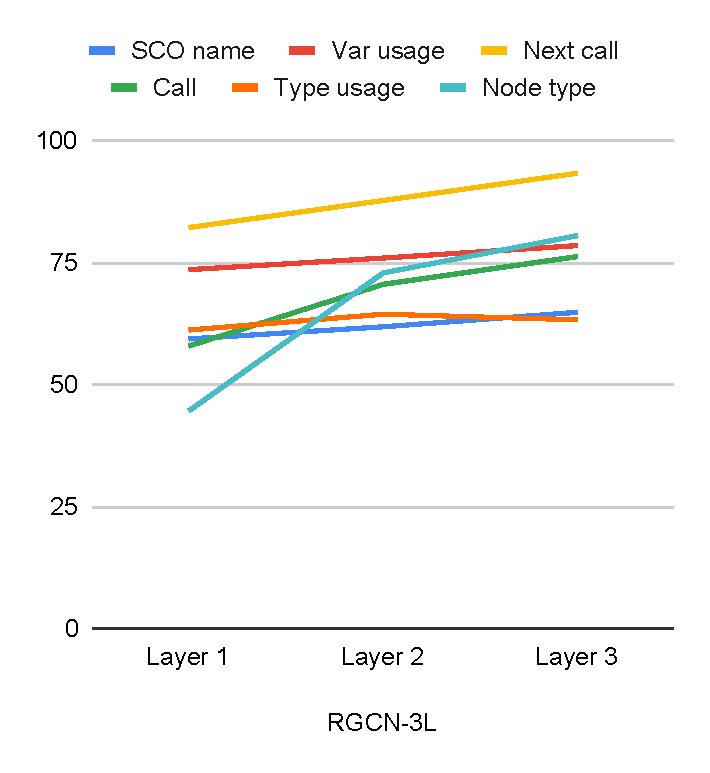
\includegraphics[width=\columnwidth]{rgcn-3l.pdf}
    \caption{Accuracy for embeddings from different layers of RGCN-3L trained on the multitask objective.}\label{fig:rgcn_layers_3}
\end{figure}

\begin{figure}[]
    \centering
    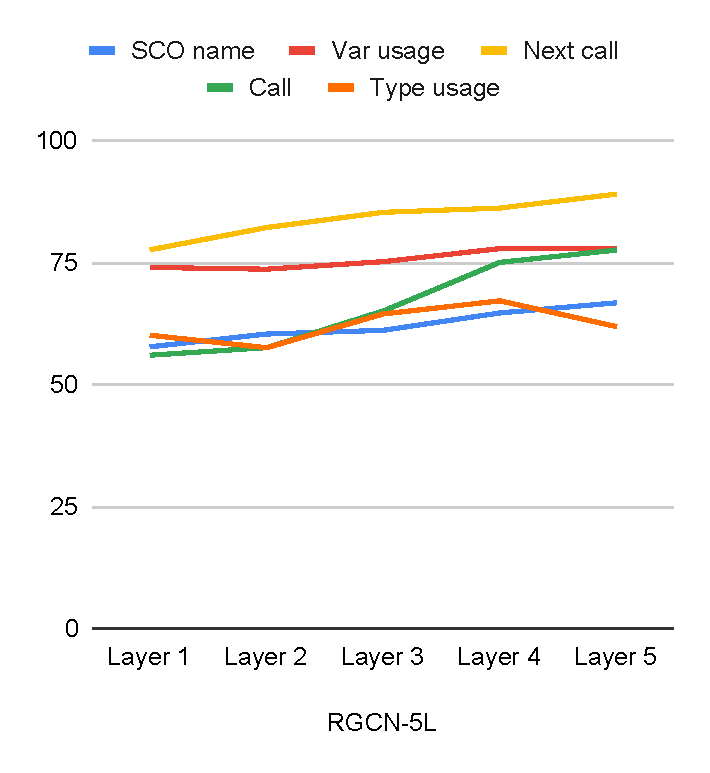
\includegraphics[width=\columnwidth]{rgcn-5l.pdf}
    \caption{Accuracy for embeddings from different layers of RGCN-5L trained on the multitask objective.}\label{fig:rgcn_layers_5}
\end{figure}

\subsection{Importance of Different Edges}

It is important to understand the contribution of different relationship types into the performance of GNN models on different objectives. We train additional models on modified versions of the original global graph, where one of the relationship types was filtered. We train these models for thirty epochs and report their final performance. 
% The results are summarized in the Table~\ref{tbl:ablation}.

We observed the most significant drop in performance after removing edges that signify that a method or function was defined inside the given class or module. Surprisingly, the performance did not suffer much after removing function call edges, although the next call prediction accuracy slightly decreased. Call edges constitute the larges proportion of all edge types (see Table~\ref{tbl:python_edge_count}). 
% The accuracy of SCO name prediction increased after removing type use edges. 
% However, it is not clear whether this result is accidental or statistically significant. 
% Removing inheritance and import edges did not affect the performance of these objectives. 

\begin{table}[]
\centering
\begin{tabular}{p{1.8cm}p{1.3cm}p{1.4cm}p{1.32cm}}
\toprule
\textbf{Filtered types} & \textbf{SCO name} & \textbf{Var usage} & \textbf{Next call} \\\midrule
Full                         & 63.49             & 78.97              & 88.31              \\\midrule
% No inheritance              & 63.86             & 79.79              & 87.17              \\\midrule
% No import                    & 63.77             & 78.91              & 87.17              \\\midrule
% No type use                  & 64.62             & 78.4               & 87.92              \\\midrule
No definitions            & 56.85             & 66.91              & 75.49              \\\midrule
No calls                     & 63.28             & 78.72              & 86.08    \\         \bottomrule
\end{tabular}
\caption{The accuracy after training GNN models on modified versions of the global graphs with one of the relationship types filtered.}
\label{tbl:ablation}
\end{table}

% \textcolor{red}{test set size}

\section{\uppercase{Discussion}}\label{sec:discuss}

\subsection{Splitting on Nodes or Edges}

During training, we used a procedure to create train and test splits. In this procedure, we divided SCO nodes into train and test groups and used these groups to generate training and testing edges. A natural alternative to this procedure is to simply split positive edges into train and test sets.

We found that the latter approach resulted in much smaller accuracy on transfer learning tasks. We explain this difference as follows. When we split positive edges into the train and test sets, the link prediction classifier does not observe all possible relationships between SCOs it encounters during training. As a consequence, these training signals are not passed onto GNN weights. The quality of GNN embeddings is dependent on the message-passing procedure. When full information about how a separate node is connected used during training, other nodes benefit from this information as well. As a result, the data splitting strategy, where all source nodes appear either in the train or test sets (but not both), results in better transfer learning performance. 

\subsection{The need for multiple splits}

In our experiments, we first perform data splits for pre-training the node representations. Then, for other experiments, we perform additional splits. 
A natural question is why all of these complex data splits necessary. In this work, we are using a GNN model to train node embeddings, which are sometimes considered as semi-supervised. All the data is present in the same graph, and training signals naturally affect even unlabeled nodes as well. For this reason, it is hard to make conclusions about the transferability of the learned embeddings. Moreover, real datasets are rarely complete. By introducing several data splits and holdout sets, we emulate the data incompleteness. This way, we can show that even when trained on an incomplete graph, node embeddings can still be useful.

\subsection{The choice of negative sampling strategy}

One of the important aspects of representation training is the negative sampling. In this work, we experimented with several negative sampling parameters. First, we tried to use uniform distribution to sample destination nodes. Our concern is that the choice of noise distribution affects the bias of the final results. The link predictor classifier can easily observe that some of the destination nodes are more popular than others. In previous works, it was shown that the distribution of SCOs indeed follows the power-law distribution, just like in the case of words in text corpora \cite{Valverde2003}. By choosing a negative sampling distribution proportional to the actual distribution of destination edges, we reduce the impact of the bias in our model. 

Another important parameter is the number of negative samples. During our experiments, we observed that the accuracy of transfer learning decreases with the increase of the number of negative samples. For this reason, we choose to use the ratio of positive to negative samples of 1.

\subsection{Evaluation approaches}

In most of our experiments, we need to predict the existence of an edge between two nodes. In general, the problem can be seen as complex given the number of possible destination nodes. In our formulation, we solve a binary classification problem. To evaluate this model, we take all the positive edges in the test split, and generate an equal amount of the negative edges. The equal proportion of the edges hints that the random baseline for accuracy should be around 0.5. However, this is not necessarily the case. 

Our goal is to evaluate embeddings. When we train a classifier, it can overfit to the destination embeddings. In case some of the destination nodes are highly connected, the classifier can predict the presence of a link whenever it sees a specific destination node. This can result in accuracy above 0.5 even when embeddings for SCOs are randomly initialized. We observe this effect in Table~\ref{tbl:transfer_results}.
% Figure~\ref{fig:transfer_gat}. 

One can argue that it is hard to interpret the accuracy measure for predicting SCO names, variable names, and next calls. A ranking measure, such as MAP can be used instead. We leave the investigation of other evaluation metrics for the future work.

\subsection{Hyper-parameter search}

In Section~\ref{sec:setup}, we mention our selected hyper parameters. This search was not arbitrary. Prior to conducting the transfer learning experiments, we performed a hyper-parameter search. Given our data and selected architectures, we found that the pre-training model performance does not grow significantly after increasing the size hidden layers beyond 100. Also, we observed that increasing the number of hidden layers does not result in significant performance improvements. For this reason, we tried to choose the number of hyper-parameters so that the training process goes faster. 

\section{\uppercase{Conclusions and Future Work}}\label{sec:conclusion}

In this paper, we conducted a series of experiments to identify the value of global relationships in the source code represented as a graph for solving several tasks. Also, we investigated the possibility of transfer learning of representation of Source Code Objects (SCOs) such as classes, function, variables, etc. We performed this analysis by first pre-training representation for nodes in the source code graph using several Graph Neural Network architectures. We used tasks such as SCO name prediction, variable usage prediction (for functions), next function call prediction as pre-training objectives. After, we evaluated the usefulness of learned embedding for solving related tasks. 

We found that different tasks for source code, such as function call prediction, node type predictions, type (class) usage predictions, are related to the objectives mentioned above. Moreover, the task of predicting next function calls yields SCO embeddings that allow predicting SCO names better than random. This suggests that some level of information about SCOs can be inferred from global relationships, and not only from specific implementations. It is worth noting, that although the performance of different models in our tests showed that the learning model can extract hidden dependencies from global graph representation, this information is likely not sufficient on its own, and can be used as augmentation for other representations. 


\bibliographystyle{apalike}
{\small
\bibliography{Splash2020.Vitaly}}

\end{document}

